\section{ТЕХНОЛОГИЯ ИССЛЕДОВАНИЯ}
Чтобы сравнение моделей между собой было более корректным, важно подобрать оптимальные параметры для дообучения каждой модели. Основными параметрами, влияющими на дообучение моделей являются learning rate (темп обучения), learning rate scheduler (изменение learning rate в процессе обучения) и weight decay (сокращение весов или $L_2$ регуляризация). Каждая модель дообучается несколько раз с различными параметрами, после чего для каждой из них выбирается наиболее оптимальный набор параметров. В качестве основной метрики для выбора лучших параметров дообучения использовалась accuracy (точность), так как в процессе анализа графиков метрик во время обучения было замечено, что micro $F_1$ и macro $F_1$ не сильно отличаются от accuracy (не более 1\%).

Все модели дообучались на 8 эпохах с ранней остановкой. Условие для ранней остановки: функция ошибки на валидационных данных не уменьшается в течение 3-х эпох.

\section{РЕЗУЛЬТАТЫ ИССЛЕДОВАНИЯ}
Для анализа и выбора оптимальных параметров будем использовать графики точности на валидационных данных в процессе обучения. На каждом рисунке 
представлены графики точности на валидационных данных во время обучения по одной модели с разными параметрами. Остальные графики (функция ошибки 
при обучении, функция ошибки на валидационных данных, micro $F_1$, macro $F_1$) можно найти в приложении \ref{app:sweeps}.
\subsection{BERT}
По графику точности, полученному в результате серии экспериментов (рисунок \ref{bert-accuracy:image}), можно сделать вывод, что наиболее 
оптимальными для дообучения BERT являются следующие параметры:
\begin{itemize}
    \item learning rate: 1,3e-4;
    \item learning rate scheduler: constant;
    \item weight decay: 7e-2.
\end{itemize}

\begin{figure}[H]
    \begin{center}
       \includegraphics[width=.8\linewidth]{bert/accuracy.png}
       \caption{График точности во время обучения BERT}
       \label{bert-accuracy:image}
    \end{center}
\end{figure}
\subsection{RoBERTa}
После дообучения серии моделей по графику точности во время обучения (рисунок \ref{roberta-accuracy:image}) можно сделать вывод, 
что оптимальными для обучения RoBERTa на текущей задаче являются параметры:
\begin{itemize}
    \item learning rate: 5e-5;
    \item learning rate scheduler: linear;
    \item wight decay: 0.
\end{itemize}
\begin{figure}[H]
    \begin{center}
       \includegraphics[width=.8\linewidth]{roberta/accuracy.png}
       \caption{График точности во время обучения RoBERTa}
       \label{roberta-accuracy:image}
    \end{center}
\end{figure}

\subsection{DistilBERT}
По графику точности во время обучения моделей (рисунок \ref{distilbert-accuracy:image}) об оптимальных параметрах обучения DistilBERT
можно сделать следующий вывод:
\begin{itemize}
    \item learning rate: 1,8e-4;
    \item learning rate scheduler: linear;
    \item weight decay: 0.
\end{itemize}
\begin{figure}[H]
    \begin{center}
       \includegraphics[width=.8\linewidth]{distilbert/accuracy.png}
       \caption{График точности во время обучения DistilBERT}
       \label{distilbert-accuracy:image}
    \end{center}
\end{figure}

\subsection{ALBERT}
Проведя анализ графика точности во время обучения моделей (рисунок \ref{albert-accuracy:image}), оптимальные параметры дообучения ALBERT были определены следующим образом:
\begin{itemize}
    \item learning rate: 5e-5;
    \item learning rate scheduler: linear;
    \item weight decay: 0.
\end{itemize}
\begin{figure}[H]
    \begin{center}
       \includegraphics[width=.8\linewidth]{albert/accuracy.png}
       \caption{График точности во время обучения ALBERT}
       \label{albert-accuracy:image}
    \end{center}
\end{figure}

\subsection{ELECTRA}
После проведения серии экспериментов по графику точности во время обучения моделей (рисунок \ref{electra-accuracy:image}) можно выбрать следующие 
оптимальные для дообучения ELECTRA параметры:
\begin{itemize}
    \item learning rate: 6,6e-5;
    \item learning rate scheduler: cosine with restarts;
    \item weight decay: 4,8e-3.
\end{itemize}
\begin{figure}[H]
    \begin{center}
       \includegraphics[width=.8\linewidth]{electra/accuracy.png}
       \caption{График точности во время обучения ELECTRA}
       \label{electra-accuracy:image}
    \end{center}
\end{figure}

\subsection{OPT}
По графику точности во время обучения моделей (рисунок \ref{opt-accuracy:image}) об оптимальности параметров дообучения OPT можно сделать 
следующий вывод:
\begin{itemize}
    \item learning rate: 5e-5;
    \item learning rate scheduler: linear;
    \item weight decay: 0.
\end{itemize}
\begin{figure}[H]
    \begin{center}
       \includegraphics[width=.8\linewidth]{opt/accuracy.png}
       \caption{График точности во время обучения OPT}
       \label{opt-accuracy:image}
    \end{center}
\end{figure}